\documentclass{article}
\usepackage[utf8]{inputenc}
\usepackage{amsmath}
\usepackage{amsfonts}
\usepackage{graphicx}


\title{LMPC theory}
\author{}
\date{October 2016}

\begin{document}

%\maketitle

\section{Closed loop LMPC}
\subsection{Main findings so far:}
\begin{itemize}
\item Current iteration data cannot be used at the end of the current iteration because the Q-function is unknown before we reach the finish line. Therefore, the safe set only contains previous laps, not even parts of the current lap.
\item The safe set should be extended beyond the finish line so that this trajectory information can be used at the end of one lap. \emph{Question: should Q be zero for all predicted states behind the finish line?}
\item Previously, all proofs were conducted assuming an infinite time problem. Can we still use this here? Is it practical to assume a finite time problem?
\end{itemize}
\subsection{Definition of periodicity}
Introduce periodicity property for the system
\begin{equation}
\dot x = f(x,u)
\end{equation}
with $x\in \mathbb{R}^n$ as states and $u\in \mathbb{R}^m$ as inputs so that
\begin{equation}\label{eq:periodicity}
f(x+P,u) = f(x,u)
\end{equation}
with $P\in \mathbb{R}^n$ is the period of the system (can be spatial but also temporal if time is a state).
From eq. \ref{eq:periodicity} one can derive the property for the discrete case:
\begin{align}
x_{k+1} &= x_k + T\cdot f(x_k,u_k)\\
x_{k+1} &= g(x_k,u_k)
\end{align}
so that
\begin{align}
g(x_k+P,u_k) &= x_k+P + T\cdot f(x_k+P,u_k)\\
g(x_k+P,u_k) &= x_k+P + T\cdot f(x_k,u_k)\\
g(x_k+P,u_k) &= g(x_k,u_k)+P
\end{align}
\emph{Important assumption:} The period $P$ is an $\mathbb{R}^n$ vector with only one non-zero element, meaning the system is periodic in only one state (e.g. the curvilinear abscissa). This makes the definition of one closed iteration easier.

\textbf{Open issue}
\begin{itemize}
\item Are there any physical examples where periodicities in multiple states make sense? This would mean that a new iteration has to be initialized whenever one of the periodic states crosses its period (e.g. 2 states: if $x_1>p_1$ or $x_2>p_2$). (This can be visually interpreted as a 2D-rectangular state space in which, whenever the trajectory reaches one of its boundaries, it appears on the opposite side). Does it affect the proofs?
\end{itemize}
\subsection{Extended safe set}
The extended safe consists of the usual safe set (all successful state trajectories) and the safe set, shifted by the period:
\[
\mathcal{SS}^j = \left\{ \bigcup_{i\in M^j} \bigcup_{t=0}^\infty \left(x_t^i\cup \left(x_t^i+P\right)\right)\right\}
\]
This extension is necessary so that trajectories can be used beyond the end of one iteration.

\textbf{Open issue:}
How is the Q-function treated in the shifted region? The shifted states should be in the terminal set so $h(x_{shifted},u)=0$ and $Q=0$. Or: Should the Q-function be "copied" to the shifted region so that $Q(x+P) = Q(x)$? In that case, we would never reach $Q=0$.

%\subsection{Iteration cost (alternative idea for Q)}
%Iteration cost (which was defined as cost to infinity before) might be redefined to allow for finite time iterations. One possible choice might be
%\begin{equation}
%J_t^j(x_t^j)=\sum_{k=t}^{t_F}h(x_k^j,u_k^j)
%\end{equation}
%with $t_F$ as the time when one iteration is finished.
%
%Is this actually necessary? Can we not prove closed iteration LMPC while still assuming infinite time cost?
\subsection{Feasibility}
Induction basis: Assume that $\mathcal{SS}^0$ is non-empty. Then at time $t=0$ of the 1st iteration the $N$ steps trajectory and its related input sequence satisfy input and state constraints $\rightarrow$ feasible (same as usual).

\begin{figure}[ht]
	\centering
	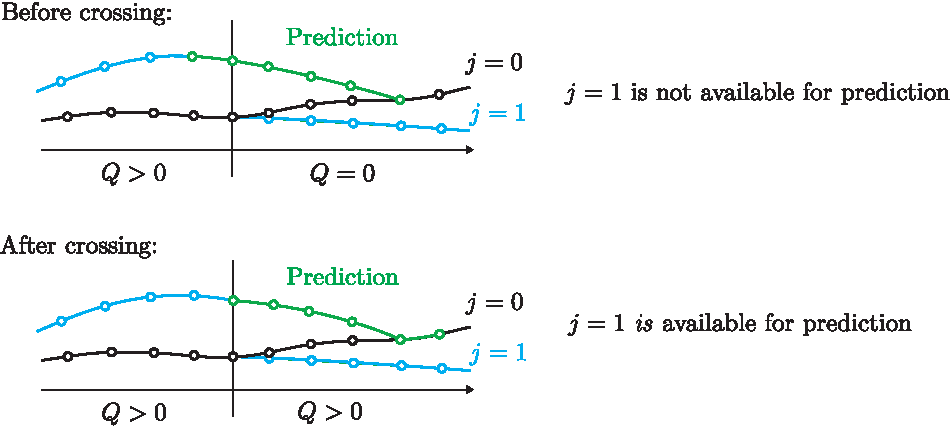
\includegraphics[width=1.0\textwidth]{../Figures/Illustrator/LMPC/Feasibility.pdf} 
	\label{fig1}
\end{figure}

\textit{Idea to prove feasibility:} Consider last state of one iteration and the subsequent state (which is the first state of the next iteration).

Consider the last state $x_t^j$ of iteration $j$ at time $t$. Assume that it is feasible so that
\begin{align}
x^* &= [x_t^*, x_{t+1}^*, ..., x_{t+N}^*]\\
u^* &= [u_t^*, u_{t+1}^*, ..., u_{t+N-1}^*]
\end{align}
is the optimal trajectory and input sequence with terminal constraint $x_{t+N}^*\in\mathcal{SS}^{j-1}$. Constraints and Q-function force $x_{t+N}^* = x_{t^*}^{i^*}$. Since $x_t^*$ is the last step within iteration $j$, all future states starting from $x_{t+1}^*$ must be in the next iteration $j+1$.

\emph{Note: What about the Q function behind the finish line?}

\emph{Next state:} At time $t+1$ we are in the $j+1$th iteration and both the state trajectory and the input sequence must satisfy input and state constraints:
\begin{align}
&[x_{t+1}^*,x_{t+2}^*,...,x_{N-1}^*, x_{t^*}^{i^*}, x_{t^*+1}^{i^*}]\\
&[u_{t+1}^*,u_{t+2}^*,...,u_{N-1}^*, u_{t^*}^{i^*}]
\end{align}
with $x_{t^*+1}^{i^*}\in\mathcal{SS}^j$.

\subsection{Asymptotic stability}
\begin{equation}\label{eq:stability}
J_{0\rightarrow N}^{*,j}(x_{t+1}^j)-J_{0\rightarrow N}^{*,j}(x_{t}^j)\leq -h(x_t^j,u_t^j)<0
\end{equation}
will still hold since it is only valid within one iteration (or does it need to be proved through iterations?).
\subsection{Convergence}
\begin{equation}
J_{0\rightarrow N}^{*,j}(x_0^j)\geq J^j
\end{equation}
will still hold since it is only based on eq. \ref{eq:stability}.\\

\textbf{But:} How can $J^{j-1}\geq J_{0\rightarrow N}^{*,j}(x_0^j)$ be proved?
\begin{align}
\sum_{t=0}^{N-1}h(x_t^{j-1},u_t^{j-1})+Q^{j-1}(x_N^{j-1})\geq\\
\min_u\left[\sum_{k=0}^{N-1}h(x_k,u_k)+Q^{j-1}(x_N)\right]
\end{align}
since $x_0^{j-1}=x_0^j$ is not necessary anymore?
%\section{Definitions}
%\subsection{Problem definition}
%Solve following problem:
%\begin{align}
%J_{0\rightarrow\infty}^*(x_S)&=\min_{\mathbf{u}}\sum_{k=0}^\infty h(x_k,u_k)\\
%\text{s.t. } x_{k+1}&=f(x_k,u_k)\\
%x_0&=x_S\\
%x_k&\in\mathcal{X},u_k\in\mathcal{U},\forall k\geq 0
%\end{align}
%with 
%\begin{align}
%h(x_F,0)&=0\\
%h(x_t^j,u_t^j)&>0\text{ } \forall \text{ } x_t^j \in \mathbb{R}^n \setminus \{x_F\},u_t^j\in\mathbb{R}^m\setminus \{0\}
%\end{align}
%and $x_F$ a feasible equilibrium:
%\[
%f(x_F,0)=0.
%\]
%
%\subsection{General definitions}
%State evolution: $x_{t+1}=f(x_t,u_t)$\\
%Cost function: $h(x_k^j,u_k^j)$ with $k$ = timestep, $j$ = iteration\\
%Iteration cost: $J_{0\rightarrow\infty}^j(x_0^j) = \sum_{k=0}^{\infty} h(x_k^j,u_k^j)$ with $x$ and $u$ are \emph{realized states}.\\
%Q-function: $Q^j(x) = \min J_{t\rightarrow\infty}^j(x)$ if $x \in \mathcal{SS}^j$\\
%Optimal cost:
%\[
%J_{0\rightarrow N}^{*,j}(x_t^j) = \min_u \left[\sum_{k=0}^{N-1}h(x_k,u_k)+Q^{j-1}(x_N)\right]
%\]
%Sampled safe set:
%\[
%\mathcal{SS}^j = \left\{ \bigcup_{i\in M^j} \bigcup_{t=0}^\infty x_t^i\right\}
%\]
%and
%\[
%M^j=\left\{ k\in [0,j]: \lim_{t\rightarrow\infty}x_t^k=x_F\right\}
%\]
%By definition, there exists a control sequence for every point in the sampled safe set that drives it to the terminal point $x_F$.

\end{document}
